\section{Introduction}\label{sec:intro}
The robot arm moved a stack of three blocks into the pyramid configuration shown in Figure~\ref{fig:blocks}.

\begin{figure}[tbph]
  \centering
  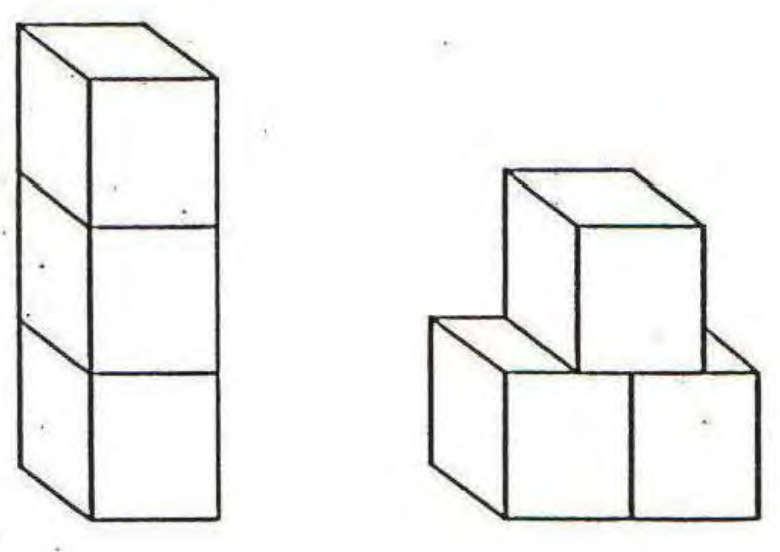
\includegraphics[width=0.4\linewidth]{graphics/blocks}
  \caption{Starting (left) and final (right) block configurations}
  \label{fig:blocks}
\end{figure}

This task was completed three times, each using a different command input method.
Starting at a known, fixed position (i.e. the \textit{hard home} of the arm), the arm is moved through space to move each block.
Critical points in the movement are marked as \textit{points} in the program.
When the program is played it runs through the entire sequence of points to move the blocks into the pyramid configuration.

The \textit{angular} input method allows each joint to be controlled independently.
Points can be created between successive joint movements but may also be combined.
The robot will execute all joint movements in parallel to transition between points.

The \textit{linear} input method allows the user to specify series of \textit{x, y, z} coordinates for the tip of the arm and the program will translate the $(x_i, y_i, z_i) \rightarrow (x_{i+1}, y_{i+1}, z_{i+1})$ spatial transition into the necessary joint movements.

Both angular and linear modes are controlled through the attached handheld controller (see Figure~\ref{fig:handheld}).

\begin{figure}[tbph]
  \centering
  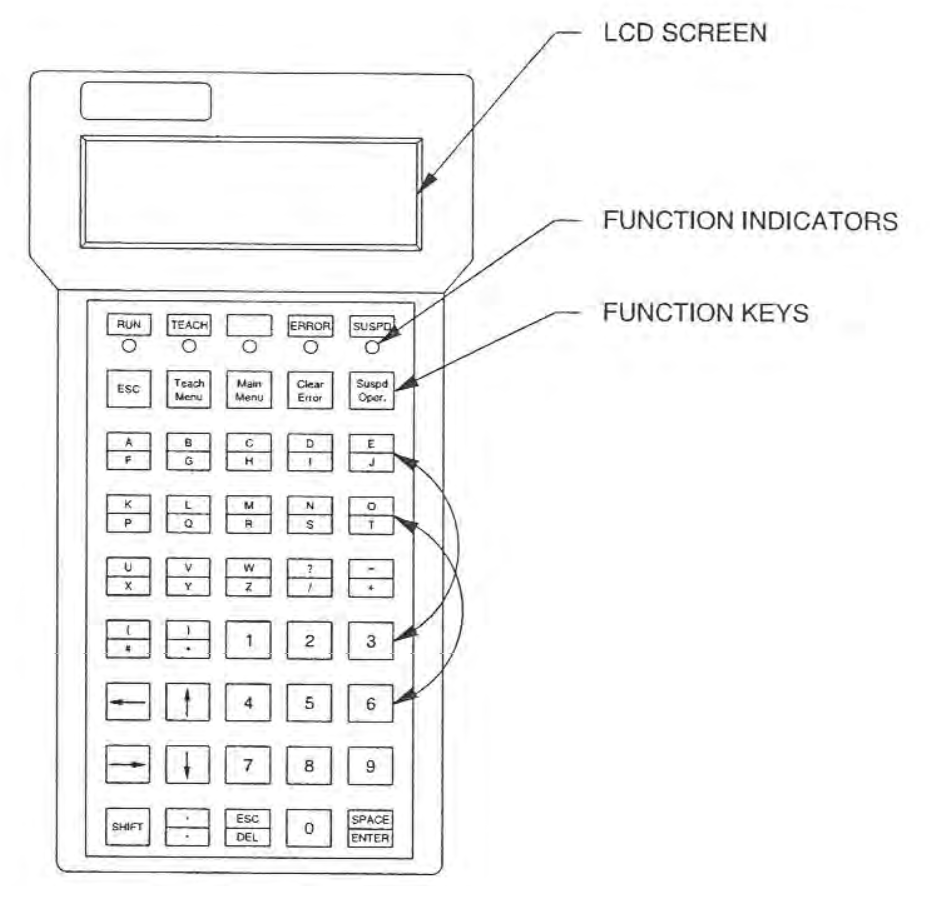
\includegraphics[width=0.4\linewidth]{graphics/handheld}
  \caption{Handheld controller for Lab-Volt 5250}
  \label{fig:handheld}
\end{figure}


\textit{GUI mode} records a sequence of joint measurements, identical to angular mode.
The GUI (see Figure~\ref{fig:gui}) provides the same functionality as the handheld controller but presents a history of the stored points on the right hand side.

\begin{figure}[tbph]
  \centering
  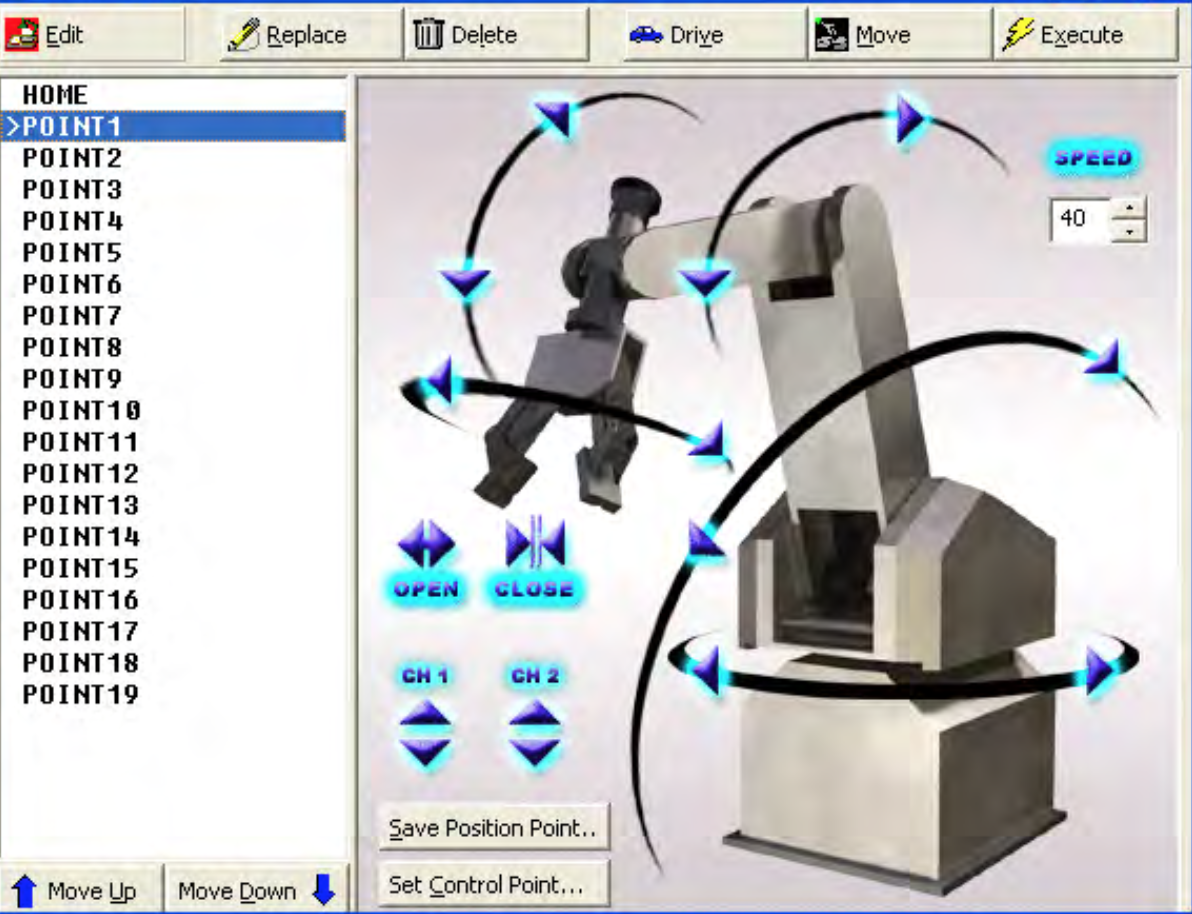
\includegraphics[width=0.4\linewidth]{graphics/gui}
  \caption{GUI for entering angular movement commands}
  \label{fig:gui}
\end{figure}

